\subsection{Tīmekļa aplikācija}
Izstrādātās tīmekļa aplikācijas galvenie elementi ir redzami \ref{orig:lapasElementi} attēlā. Attēla kreisajā pusē ir redzams \texttt{svg} elements, uz kura lietotājs var zīmēt savu izvēlēto ciparu. Zem šī elementa ir pogas ar papildus funkcijām (\ref{orig:svgElementi} attēls). Uzspiežot pogu 'GUESS', zīmējums tiek saglabāts, analizēts un rezultāts ar zīmējuma samazināto versiju ir redzams attēla labajā pusē.

\begin{figure}[H]
    \centering
    \fbox{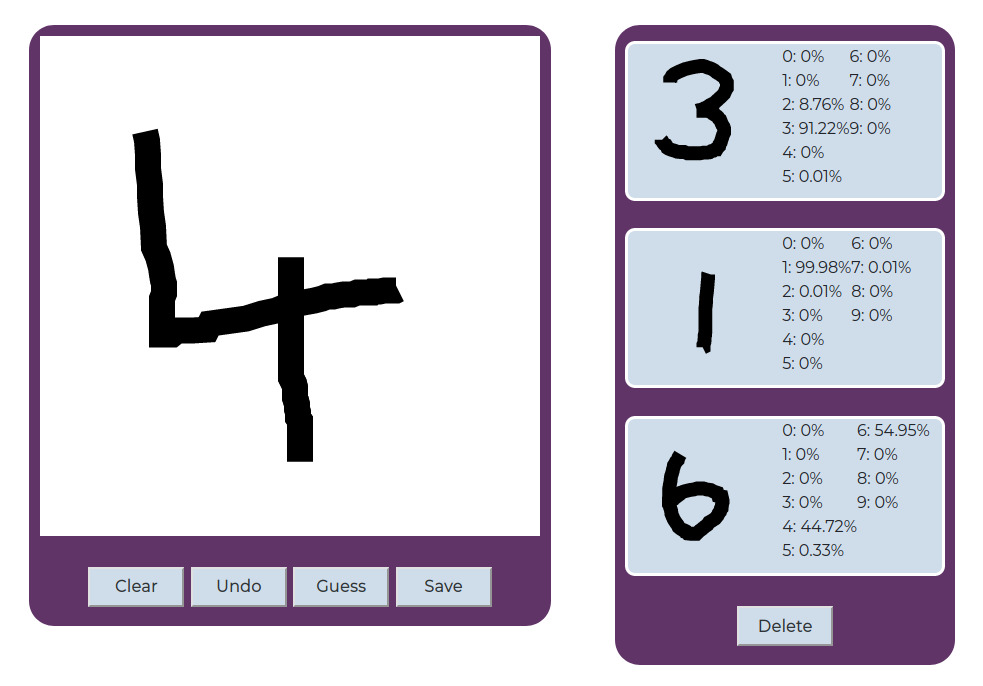
\includegraphics[width=120mm]{history.jpeg}}
    \caption{Tīmekļa aplikācijas elementi}
    \label{orig:lapasElementi}
\end{figure}

\begin{figure}[H]
    \centering
    \fbox{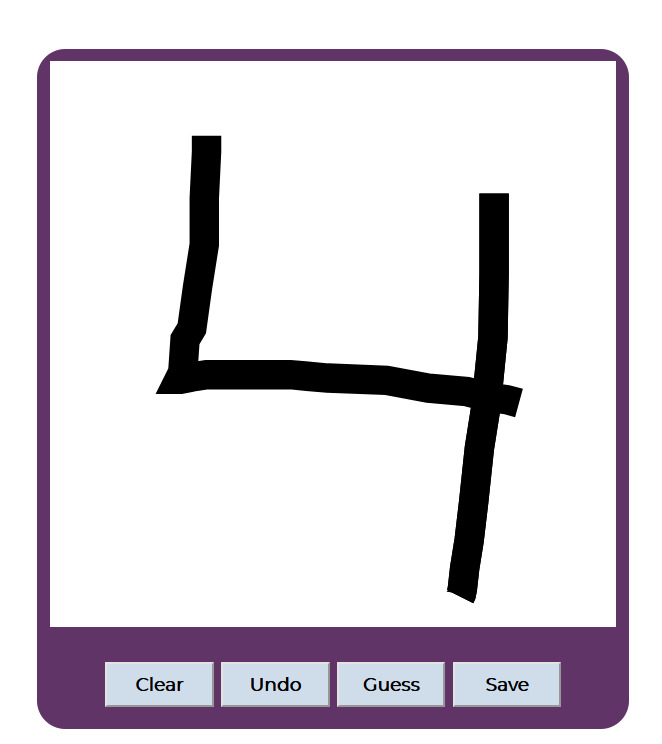
\includegraphics[width=120mm]{drawing.jpeg}}
    \caption{Galvenais svg elements un pogas}
    \label{orig:svgElementi}
\end{figure}

\par Zīmējumu vēstures skats ir redzams \ref{orig:selection} attēla labajā pusē. Sarakstam ir pielietota iespēja izvēlēties kādu no elementiem un izdzēst to no vēstures.

\begin{figure}[H]
    \centering
    \fbox{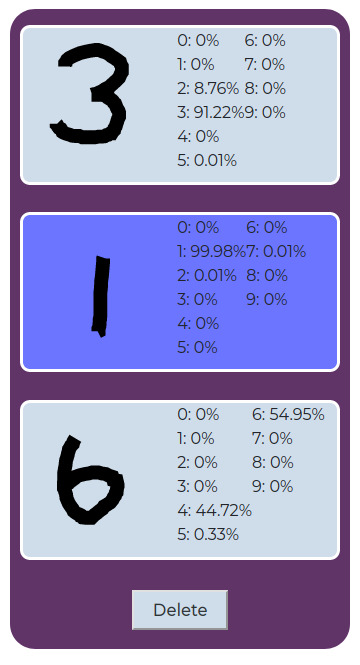
\includegraphics[width=120mm]{selection.jpeg}}
    \caption{Zīmējumu vēsture}
    \label{orig:selection}
\end{figure}

\par Viena no zīmējumam pievienotajām funckijām ir attēla saglabāšana. Tā tiek pielietota, lietotājam nospiežot 'SAVE' pogu, kas redzama \ref{orig:svgElementi} attēlā. Ar šo pogu zīmējums tiek saglabāts kā png fails lietotāja datorā ar nosaukumu \textit{number.png}. \ref{orig:downloadedFile} attēlā redzams lejupielādētais zīmējums.
\begin{figure}[H]
    \centering
    \fbox{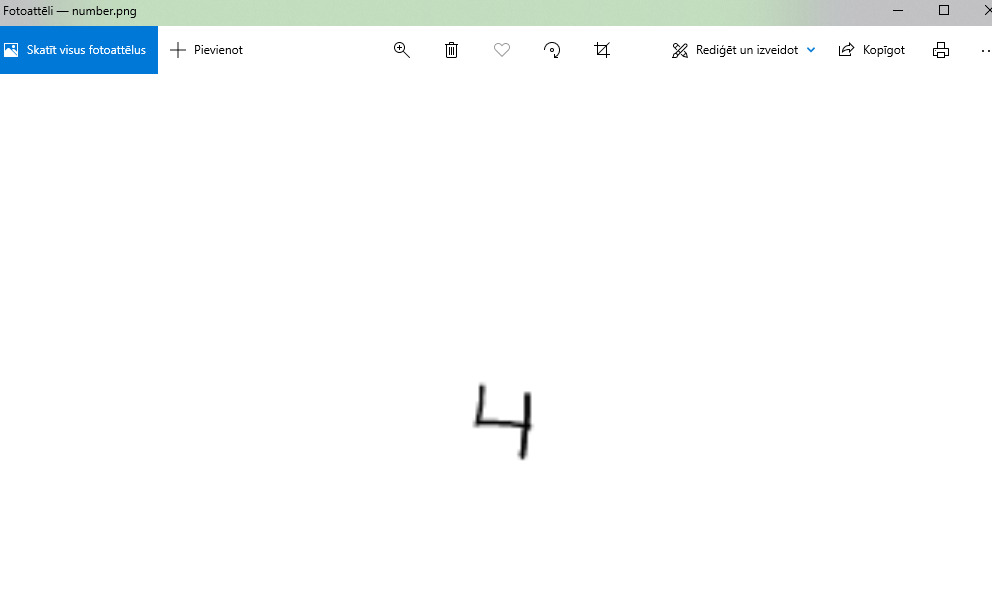
\includegraphics[width=120mm]{downloaded.jpeg}}
    \caption{Lejupielādētais attēls}
    \label{orig:downloadedFile}
\end{figure}
